% !TeX program = xelatex
\documentclass[aspectratio=169,11pt]{beamer}

% -------------------------------------------------
% Packages
% -------------------------------------------------
\usepackage{kotex}
\usepackage{fontspec}
\usepackage{amsmath,amssymb,bm,mathtools}
\usepackage{booktabs,array}
\usepackage{xcolor}
\usepackage{colortbl}
\usepackage{tikz}
\usetikzlibrary{positioning,arrows.meta,calc,fit,decorations.pathreplacing}
\usepackage[most]{tcolorbox}
\usepackage{listings}
\usepackage{adjustbox}

% -------------------------------------------------
% Colors (same as the notes)
% -------------------------------------------------
\definecolor{deepblue}{RGB}{34,71,120}
\definecolor{softblue}{RGB}{239,246,253}
\definecolor{softgray}{RGB}{246,247,249}
\definecolor{softgreen}{RGB}{239,249,242}
\definecolor{softyellow}{RGB}{255,249,229}
\definecolor{codegray}{RGB}{248,248,248}

% -------------------------------------------------
% Beamer look
% -------------------------------------------------
\usetheme{default}
\usefonttheme[onlymath]{serif}
\setbeamertemplate{navigation symbols}{}
\setbeamersize{text margin left=8mm,text margin right=8mm}
\setbeamercolor{structure}{fg=deepblue}
\setbeamercolor{frametitle}{fg=deepblue}
\setbeamercolor{title}{fg=deepblue}
\setbeamerfont{frametitle}{size=\large,series=\bfseries}
\setbeamertemplate{itemize items}[circle]
\setbeamertemplate{enumerate items}[default]
\setbeamertemplate{frametitle}{%
  \vskip3mm
  {\usebeamerfont{frametitle}\usebeamercolor[fg]{frametitle}\insertframetitle\par}%
  \vskip1mm
  {\color{deepblue!45}\hrule height 0.6pt}%
  \vskip1mm}
\setbeamertemplate{footline}{%
  \hbox to\paperwidth{%
    \hspace*{8mm}{\color{black!45}\scriptsize PyTorch 입문\ifx\insertsectionhead\empty\else\ \ $\cdot$\ \ \insertsectionhead\fi}%
    \hfill{\color{black!45}\scriptsize\insertframenumber\,/\,\inserttotalframenumber}\hspace*{8mm}}%
  \vskip2.5mm}
\setbeamertemplate{title page}{%
  \vfill
  \begin{center}
  {\color{deepblue}\Huge\bfseries\inserttitle\par}
  \vskip3mm
  {\color{deepblue!60}\rule{9cm}{0.8pt}\par}
  \vskip3mm
  {\large\insertsubtitle\par}
  \vskip8mm
  {\normalsize\insertdate\par}
  \end{center}
  \vfill}
\AtBeginSection[]{%
  \begin{frame}
  \vfill
  \centering
  {\color{deepblue!55}\Large\bfseries \insertsectionnumber\par}
  \vskip2mm
  {\color{deepblue}\LARGE\bfseries\insertsectionhead\par}
  \vskip3mm
  {\color{deepblue!50}\rule{7cm}{0.8pt}\par}
  \vfill
  \end{frame}}
\setlength{\leftmargini}{1.2em}
\setlength{\leftmarginii}{1.1em}

% -------------------------------------------------
% Boxes (same colors as the notes)
% -------------------------------------------------
\newtcolorbox{keybox}[1][]{colback=softblue,colframe=deepblue,boxrule=0.7pt,arc=2mm,
  title=#1,fonttitle=\bfseries\small,left=2mm,right=2mm,top=1mm,bottom=1mm,
  toptitle=0.5mm,bottomtitle=0.5mm}
\newtcolorbox{thinkbox}[1][]{colback=softyellow,colframe=orange!70!black,boxrule=0.6pt,arc=2mm,
  title=#1,fonttitle=\bfseries\small,left=2mm,right=2mm,top=1mm,bottom=1mm,
  toptitle=0.5mm,bottomtitle=0.5mm}
\newtcolorbox{remarkbox}[1][]{colback=softgray,colframe=black!45,boxrule=0.5pt,arc=2mm,
  title=#1,fonttitle=\bfseries\small,left=2mm,right=2mm,top=1mm,bottom=1mm,
  toptitle=0.5mm,bottomtitle=0.5mm}

% -------------------------------------------------
% Code style
% -------------------------------------------------
\lstdefinestyle{pythonstyle}{
  language=Python,
  backgroundcolor=\color{codegray},
  basicstyle=\ttfamily\scriptsize,
  keywordstyle=\bfseries\color{deepblue},
  commentstyle=\itshape\color{black!55},
  stringstyle=\color{black!75},
  numbers=none,
  frame=single,
  rulecolor=\color{black!25},
  breaklines=true,
  showstringspaces=false,
  tabsize=4,
  columns=fullflexible,
  keepspaces=true,
  aboveskip=1mm,
  belowskip=1mm
}
\lstset{style=pythonstyle}
% program output: no Python colors, light green background
\lstdefinestyle{outstyle}{style=pythonstyle,language={},backgroundcolor=\color{softgreen}}

% -------------------------------------------------
% Math commands (same as the notes)
% -------------------------------------------------
\newcommand{\R}{\mathbb{R}}
\newcommand{\vect}[1]{\bm{#1}}
\newcommand{\T}{^{\mathsf T}}
\newcommand{\pd}[2]{\frac{\partial #1}{\partial #2}}

\newcommand{\figcap}[1]{\par\vskip1mm{\centering\footnotesize\color{black!70}#1\par}}
\newcommand{\code}[1]{\texttt{#1}}

\graphicspath{{slides_figures/}}

\title{PyTorch 입문}
\subtitle{텐서 $\cdot$ 자동 미분 $\cdot$ \texttt{nn} $\cdot$ \texttt{optim} $\cdot$ \texttt{utils.data} $\cdot$ MNIST 분류 코드 읽기}
\date{딥러닝개론및연습 $\cdot$ 2026년 2학기}

\begin{document}

% =================================================
\begin{frame}[plain]
\titlepage
\end{frame}

% =================================================
\begin{frame}{이번 시간의 핵심 질문}
\begin{keybox}[이번 시간의 핵심 질문]
\begin{itemize}
\item 지금까지 우리는 NumPy로 \textbf{모든 것을 직접} 만들었다: 계층의 순전파와 역전파, 기울기 갱신, 미니배치 나누기
\item 새로운 계층을 쓸 때마다 역전파 식을 \textbf{손으로 유도}해야 할까?
\item 수십만 장의 이미지와 수백만 개의 매개변수를 \textbf{GPU}로 빠르게 계산하려면?
\item 실제 연구와 산업에서는 신경망을 어떤 도구로 만들까?
\end{itemize}
\end{keybox}
\vskip2mm
\begin{center}
\large $\Rightarrow$ \textbf{딥러닝 프레임워크: PyTorch}
\end{center}
\end{frame}

\begin{frame}{학습목표}
\begin{enumerate}
\item PyTorch가 무엇이고, 무엇을 대신해 주는지 설명할 수 있다
\item 텐서(tensor)를 만들고 shape, dtype, device를 다룰 수 있다
\item 자동 미분(autograd)이 우리가 배운 역전파와 같은 일을 한다는 것을 확인한다
\item \code{torch.nn}으로 모델을, \code{torch.optim}으로 갱신 규칙을 만든다
\item \code{torch.utils.data}의 \code{Dataset}, \code{DataLoader}로 미니배치를 만든다
\item 학습 루프의 5줄(순전파 $\to$ 손실 $\to$ 기울기 초기화 $\to$ 역전파 $\to$ 갱신)을 이해한다
\item MNIST 분류 코드 \code{mnist\_torch.py}를 처음부터 끝까지 읽고 실행한다
\end{enumerate}
\end{frame}

\begin{frame}{목차}
\small
\tableofcontents
\end{frame}

% =================================================
\section{PyTorch란 무엇인가}
% =================================================

\begin{frame}{지금까지 우리가 직접 만든 것}
\centering
\small
\renewcommand{\arraystretch}{1.25}
\begin{tabular}{>{\raggedright}p{3.2cm}>{\raggedright}p{5.2cm}>{\raggedright\arraybackslash}p{4.6cm}}
\toprule
\textbf{할 일} & \textbf{NumPy로 직접 만든 것} & \textbf{어려운 점} \\
\midrule
데이터 저장, 계산 & \code{np.array}, \code{X @ W + B} & CPU에서만 계산 \\
계층 & \code{Affine}, \code{Relu}, \code{Convolution}, \ldots{} 의 \code{forward} & 계층마다 클래스 작성 \\
역전파 & 각 계층의 \code{backward} & 식을 \textbf{손으로 유도}, 틀리기 쉬움 (기울기 검사) \\
매개변수 갱신 & \code{SGD}, \code{Momentum}, \code{Adam} 클래스 & 매개변수 딕셔너리 관리 \\
미니배치 & \code{np.random.permutation}으로 섞고 자르기 & 매번 같은 코드 반복 \\
\bottomrule
\end{tabular}
\vskip3mm
\raggedright
\begin{itemize}
\item 원리를 이해하려면 직접 만드는 것이 가장 좋다. \textbf{그래서 지금까지 직접 만들었다.}
\item 하지만 큰 모델을 실제로 학습할 때 이것을 매번 직접 짤 수는 없다.
\end{itemize}
\end{frame}

\begin{frame}{딥러닝 프레임워크}
\begin{itemize}
\item \textbf{딥러닝 프레임워크}: 위의 일들을 미리 만들어 둔 라이브러리
\begin{itemize}
\item \textbf{PyTorch} (2016, Meta AI에서 시작 $\to$ 현재 Linux 재단 산하 PyTorch Foundation)
\item TensorFlow / Keras (2015, Google), JAX (Google)
\end{itemize}
\item 현재 연구 논문과 공개 모델(예: Hugging Face의 언어 모델들)의 대부분이 \textbf{PyTorch}로 작성된다
\item Python 코드처럼 \textbf{한 줄씩 실행}되므로 NumPy를 아는 사람이 배우기 쉽다
\end{itemize}
\vskip2mm
\begin{keybox}[PyTorch를 한 문장으로]
\textbf{GPU에서 동작하고, 기울기를 자동으로 계산하는 NumPy} \;+\; 신경망 부품 모음
\end{keybox}
\end{frame}

\begin{frame}{PyTorch의 구성: 이번 시간에 배울 다섯 가지}
\centering
\small
\renewcommand{\arraystretch}{1.3}
\begin{tabular}{>{\raggedright}p{3.0cm}>{\raggedright}p{5.4cm}>{\raggedright\arraybackslash}p{4.4cm}}
\toprule
\textbf{모듈} & \textbf{역할} & \textbf{우리 코드에서 대신하는 것} \\
\midrule
\code{torch} & \textbf{텐서}: GPU에서도 계산되는 다차원 배열 & \code{np.array}, \code{np.exp}, \ldots \\
\code{torch.autograd} & \textbf{자동 미분}: \code{loss.backward()} 한 줄로 모든 기울기 계산 & 모든 \code{backward} \\
\code{torch.nn} & 계층, 모델, 손실 함수 & \code{Affine}, \code{Relu}, \code{SoftmaxWithCrossEntropy} \\
\code{torch.optim} & 매개변수 갱신 규칙 & \code{optimizers.py} \\
\code{torch.utils.data} & 데이터 묶음, 미니배치 & \code{permutation}으로 섞고 자르기 \\
\bottomrule
\end{tabular}
\vskip3mm
\raggedright
\begin{itemize}
\item \code{torch}가 라이브러리 전체이고, \code{nn}, \code{optim}, \code{utils.data}는 그 안의 \textbf{하위 모듈}이다
\item NumPy에 \code{numpy.linalg}, \code{numpy.random}이 있는 것과 같다. 따로 설치할 필요가 없다
\end{itemize}
\end{frame}

\begin{frame}[fragile]{설치와 확인}
\begin{itemize}
\item 설치 (CPU 버전): \code{pip install torch}
\item GPU(NVIDIA CUDA)용은 \code{pytorch.org}에서 자기 환경에 맞는 설치 명령을 골라 쓴다
\item Google Colab에는 이미 설치되어 있고, GPU도 무료로 쓸 수 있다
\end{itemize}
\begin{lstlisting}
import torch
print("torch version:", torch.__version__)
print("GPU available:", torch.cuda.is_available())
\end{lstlisting}
\begin{lstlisting}[style=outstyle]
torch version: 2.14.1+cpu
GPU available: False
\end{lstlisting}
\begin{itemize}
\item 이 강의의 모든 결과는 GPU 없이 \textbf{CPU}로 실행한 것이다. MNIST 정도는 CPU로 충분하다
\item 예제 코드: \code{torch\_basics.py} (이번 시간의 작은 예제 모음), \code{mnist\_torch.py}
\end{itemize}
\end{frame}

% =================================================
\section{텐서 (Tensor)}
% =================================================

\begin{frame}[fragile]{텐서 만들기}
\begin{itemize}
\item \textbf{텐서}: PyTorch의 다차원 배열. NumPy의 \code{ndarray}와 거의 같다
\end{itemize}
\begin{columns}[T,onlytextwidth]
\begin{column}{0.47\textwidth}
\begin{lstlisting}
a = torch.tensor([[1., 2., 3.],
                  [4., 5., 6.]])
print(a)
print(a.shape, a.dtype, a.device)

print(torch.zeros(2, 3))
print(torch.arange(6).reshape(2, 3))
print(torch.randn(2, 3))   # N(0, 1)
\end{lstlisting}
\end{column}
\begin{column}{0.49\textwidth}
\begin{lstlisting}[style=outstyle]
tensor([[1., 2., 3.],
        [4., 5., 6.]])
torch.Size([2, 3]) torch.float32 cpu
tensor([[0., 0., 0.],
        [0., 0., 0.]])
tensor([[0, 1, 2],
        [3, 4, 5]])
tensor([[ 1.5410, -0.2934, -2.1788],
        [ 0.5684, -1.0845, -1.3986]])
\end{lstlisting}
\end{column}
\end{columns}
\vskip1mm
\begin{itemize}
\item 모든 텐서는 세 가지 속성을 가진다: \textbf{\code{shape}} (모양), \textbf{\code{dtype}} (자료형), \textbf{\code{device}} (CPU / GPU)
\item \code{torch.zeros(2, 3)}: NumPy의 \code{np.zeros((2, 3))}와 달리 괄호를 하나 덜 써도 된다
\end{itemize}
\end{frame}

\begin{frame}{자료형 (dtype)}
\centering
\footnotesize
\renewcommand{\arraystretch}{1.2}
\begin{tabular}{lll}
\toprule
\textbf{dtype} & \textbf{쓰는 곳} & \textbf{만들어지는 경우} \\
\midrule
\code{torch.float32} (\code{float}) & 입력 데이터, 가중치 & \code{torch.tensor([1., 2.])} (기본값) \\
\code{torch.int64} (\code{long}) & \textbf{클래스 번호} (정답 레이블) & \code{torch.tensor([3, 7])} \\
\code{torch.float64} (\code{double}) & 거의 쓰지 않는다 & NumPy 배열을 그대로 변환할 때 \\
\bottomrule
\end{tabular}
\vskip2mm
\raggedright
\small
\begin{itemize}
\item NumPy의 기본은 \code{float64}, PyTorch의 기본은 \code{float32}: 메모리가 절반이고 GPU에서 훨씬 빠르다. 정밀도는 신경망 학습에 충분하다
\item 자료형이 섞이면 \textbf{오류}가 난다. 초보자가 가장 많이 만나는 오류 두 가지:
\end{itemize}
\begin{remarkbox}[자주 보는 오류]
\footnotesize
\code{mat1 and mat2 must have the same dtype, but got Double and Float}\\
\quad $\to$ \code{float64} 입력을 \code{float32} 가중치에 넣었다. \code{dtype=torch.float32}로 변환\\[0.5mm]
\code{expected target dtype to be Long or Byte, but got Float}\\
\quad $\to$ 손실 함수의 정답 레이블은 \code{int64}여야 한다
\end{remarkbox}
\end{frame}

\begin{frame}[fragile]{NumPy와 오가기}
\begin{columns}[T,onlytextwidth]
\begin{column}{0.52\textwidth}
\begin{lstlisting}
x_np = np.array([1.0, 2.0, 3.0])   # float64
x_t = torch.tensor(x_np)
print(x_t, x_t.dtype)
print(torch.tensor(x_np, dtype=torch.float32))
print(a.numpy())
\end{lstlisting}
\end{column}
\begin{column}{0.44\textwidth}
\begin{lstlisting}[style=outstyle]
tensor([1., 2., 3.], dtype=torch.float64)
  torch.float64
tensor([1., 2., 3.])
[[1. 2. 3.]
 [4. 5. 6.]]
\end{lstlisting}
\end{column}
\end{columns}
\vskip2mm
\begin{itemize}
\item \code{torch.tensor(x\_np)}: NumPy의 \code{float64}를 \textbf{그대로} 가져온다 $\to$ \code{dtype=torch.float32}를 붙인다
\item \code{tensor.numpy()}: 다시 NumPy 배열로 (그림 그리기, 결과 저장 등)
\begin{itemize}
\item GPU에 있는 텐서는 먼저 \code{.cpu()}로 가져와야 한다
\item 기울기를 추적 중인 텐서는 \code{.detach().numpy()}
\end{itemize}
\item 원소 하나짜리 텐서 $\to$ Python 숫자: \code{.item()} (예: \code{loss.item()})
\end{itemize}
\end{frame}

\begin{frame}[fragile]{연산: NumPy와 거의 같다}
\begin{columns}[T,onlytextwidth]
\begin{column}{0.47\textwidth}
\begin{lstlisting}
W = torch.ones(3, 4)
print(a @ W)               # (2,3)@(3,4)
b = torch.tensor([1., 2., 3.])
print(a + 10 * b)          # broadcasting
print(a.sum(dim=0))
print(a.sum(dim=1))
print(a.argmax(dim=1))
print(a[1, 2], a[1, 2].item())
\end{lstlisting}
\end{column}
\begin{column}{0.49\textwidth}
\begin{lstlisting}[style=outstyle]
tensor([[ 6.,  6.,  6.,  6.],
        [15., 15., 15., 15.]])
tensor([[11., 22., 33.],
        [14., 25., 36.]])
tensor([5., 7., 9.])
tensor([ 6., 15.])
tensor([2, 2])
tensor(6.) 6.0
\end{lstlisting}
\end{column}
\end{columns}
\vskip2mm
\begin{itemize}
\item 행렬곱 \code{@}, 원소별 연산, \textbf{브로드캐스팅}, 인덱싱, \code{.T}, \code{reshape}: NumPy와 같다
\item 차이: NumPy의 \code{axis} 대신 \textbf{\code{dim}}을 쓴다 (\code{axis}도 받아 주지만 \code{dim}이 표준)
\end{itemize}
\end{frame}

\begin{frame}{NumPy $\leftrightarrow$ PyTorch 대응표}
\centering
\footnotesize
\renewcommand{\arraystretch}{1.2}
\begin{tabular}{ll}
\toprule
\textbf{NumPy} & \textbf{PyTorch} \\
\midrule
\code{np.array(L)} & \code{torch.tensor(L)} \\
\code{np.zeros((2, 3))}, \code{np.ones((2, 3))} & \code{torch.zeros(2, 3)}, \code{torch.ones(2, 3)} \\
\code{np.random.randn(2, 3)} & \code{torch.randn(2, 3)} \\
\code{np.random.seed(0)} & \code{torch.manual\_seed(0)} \\
\code{x.sum(axis=0, keepdims=True)} & \code{x.sum(dim=0, keepdim=True)} \\
\code{np.argmax(x, axis=1)} & \code{x.argmax(dim=1)} \\
\code{np.exp(x)}, \code{np.log(x)}, \code{np.maximum(0, x)} & \code{torch.exp(x)}, \code{torch.log(x)}, \code{torch.relu(x)} \\
\code{np.concatenate([x, y])} & \code{torch.cat([x, y])} \\
\code{x.astype(np.float32)} & \code{x.float()} \ 또는 \ \code{x.to(torch.float32)} \\
\code{x.size} (원소 수) & \code{x.numel()} \\
\code{x.shape}, \code{x.T}, \code{x @ W}, \code{x.reshape(3, 2)} & 같음 \\
\bottomrule
\end{tabular}
\end{frame}

\begin{frame}[fragile]{device: CPU와 GPU}
\begin{itemize}
\item 텐서는 \textbf{CPU 메모리} 또는 \textbf{GPU 메모리}에 있다 (\code{a.device})
\item \code{.to(device)}로 옮긴다. GPU에 있는 텐서끼리의 연산은 GPU에서 병렬로 실행된다
\end{itemize}
\begin{lstlisting}
device = "cuda" if torch.cuda.is_available() else "cpu"   # GPU if we have one
x = x.to(device)              # data to the device
model = model.to(device)      # all parameters of the model to the device
\end{lstlisting}
\begin{keybox}[규칙]
\textbf{함께 계산하는 텐서는 모두 같은 device에 있어야 한다.}
모델을 GPU로 보냈으면 입력 미니배치도 GPU로 보낸다.
\end{keybox}
\begin{itemize}
\item 이렇게 써 두면 \textbf{같은 코드}가 GPU가 있으면 GPU로, 없으면 CPU로 돈다
\item GPU가 빠른 이유: 행렬곱의 곱셈과 덧셈이 서로 독립이라 동시에 계산할 수 있다
\end{itemize}
\end{frame}

% =================================================
\section{자동 미분 (Autograd)}
% =================================================

\begin{frame}[fragile]{핵심 아이디어: 순전파가 계산 그래프를 기록한다}
\begin{columns}[T,onlytextwidth]
\begin{column}{0.50\textwidth}
\begin{lstlisting}
x = torch.tensor(2.0, requires_grad=True)
y = x ** 2 + 3 * x      # forward
y.backward()            # backward
print(y.item(), x.grad.item())
\end{lstlisting}
\begin{lstlisting}[style=outstyle]
10.0 7.0
\end{lstlisting}
\small
\begin{itemize}
\item \code{requires\_grad=True}: ``이 텐서에 대한 미분이 필요하다''
\item 순전파를 하는 동안 PyTorch가 \textbf{계산 그래프}를 기록
\item \code{y.backward()}: 그래프를 거꾸로 따라가며 \textbf{연쇄법칙} 적용
\item 결과는 \code{x.grad}에 저장: $\dfrac{dy}{dx}=2x+3=7$
\end{itemize}
\end{column}
\begin{column}{0.47\textwidth}
\centering
\begin{adjustbox}{max width=\linewidth}
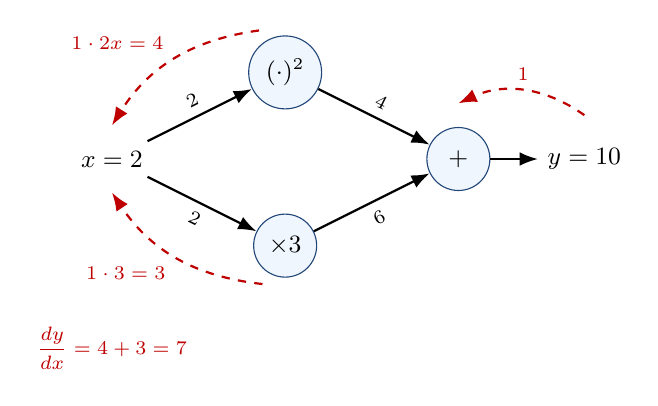
\begin{tikzpicture}[>=Latex,
  op/.style={circle,draw=deepblue,fill=softblue,minimum size=8mm,font=\small},
  vr/.style={font=\small}]
\node[vr] (x) at (0,0) {$x=2$};
\node[op] (sq) at (2.2,1.1) {$(\cdot)^2$};
\node[op] (m3) at (2.2,-1.1) {$\times3$};
\node[op] (pl) at (4.4,0) {$+$};
\node[vr] (y) at (6.0,0) {$y=10$};
\draw[->,thick] (x) -- node[above,sloped,font=\scriptsize]{2} (sq);
\draw[->,thick] (x) -- node[below,sloped,font=\scriptsize]{2} (m3);
\draw[->,thick] (sq) -- node[above,sloped,font=\scriptsize]{4} (pl);
\draw[->,thick] (m3) -- node[below,sloped,font=\scriptsize]{6} (pl);
\draw[->,thick] (pl) -- (y);
% backward
\draw[->,red!75!black,thick,dashed] ([yshift=2mm]sq.north west) to[bend right=25] node[above left,font=\scriptsize]{$1\cdot2x=4$} ([yshift=2mm]x.north);
\draw[->,red!75!black,thick,dashed] ([yshift=-2mm]m3.south west) to[bend left=25] node[below left,font=\scriptsize]{$1\cdot3=3$} ([yshift=-2mm]x.south);
\draw[->,red!75!black,thick,dashed] ([yshift=3mm]y.north) to[bend right=30] node[above,font=\scriptsize]{$1$} ([yshift=3mm]pl.north);
\node[font=\scriptsize,red!75!black] at (0,-2.4) {$\dfrac{dy}{dx}=4+3=7$};
\end{tikzpicture}
\end{adjustbox}
\figcap{검은 화살표: 순전파 (값), 빨간 점선: 역전파 (기울기)}
\end{column}
\end{columns}
\end{frame}

\begin{frame}[fragile]{우리가 유도한 역전파 식과 비교}
\begin{itemize}
\item Affine 계층 $A=XW+B$, 손실 $L=\tfrac12\sum(A-T)^2$. 우리가 유도한 식: $\pd{L}{W}=X\T\pd{L}{A}$, \ $\pd{L}{B}=\sum_{\text{행}}\pd{L}{A}$
\end{itemize}
\begin{lstlisting}
X = torch.tensor([[1., 2.], [3., 4.]])
W = torch.tensor([[0.5], [-1.0]], requires_grad=True)
B = torch.tensor([[0.1]], requires_grad=True)
T = torch.tensor([[1.], [0.]])
A = X @ W + B
L = 0.5 * ((A - T) ** 2).sum()
L.backward()                               # autograd
dA = (A - T).detach()                      # dL/dA, by hand
print(W.grad.T, (X.T @ dA).T)
print(B.grad, dA.sum(dim=0, keepdim=True))
\end{lstlisting}
\begin{lstlisting}[style=outstyle]
tensor([[ -9.6000, -14.4000]]) tensor([[ -9.6000, -14.4000]])
tensor([[-4.8000]]) tensor([[-4.8000]])
\end{lstlisting}
\begin{itemize}
\item 정확히 같다. \textbf{우리가 계층마다 손으로 짠 \code{backward}를 autograd가 대신 해 준다}
\end{itemize}
\end{frame}

\begin{frame}[fragile]{주의 1: 기울기는 더해진다 $\to$ 매번 0으로}
\begin{columns}[T,onlytextwidth]
\begin{column}{0.52\textwidth}
\begin{lstlisting}
x = torch.tensor(2.0, requires_grad=True)
for k in range(3):
    (x ** 2).backward()      # d/dx = 2x = 4
    print(x.grad.item())
x.grad.zero_()
print(x.grad.item())
\end{lstlisting}
\end{column}
\begin{column}{0.44\textwidth}
\begin{lstlisting}[style=outstyle]
4.0
8.0
12.0
0.0
\end{lstlisting}
\end{column}
\end{columns}
\vskip2mm
\begin{itemize}
\item \code{backward()}는 기울기를 \code{.grad}에 \textbf{덮어쓰지 않고 더한다}
(한 변수가 여러 경로로 쓰이면 모든 경로의 기울기를 더해야 하기 때문)
\item 따라서 미니배치마다 \code{backward()} \textbf{전에} 기울기를 0으로: 학습 코드의 \code{optimizer.zero\_grad()}
\end{itemize}
\begin{thinkbox}[잊으면?]
이전 미니배치들의 기울기가 계속 쌓여서 엉뚱한 방향으로 갱신된다. 오류 메시지도 나지 않으므로 찾기 어렵다.
\end{thinkbox}
\end{frame}

\begin{frame}[fragile]{주의 2: 기울기가 필요 없을 때는 \code{torch.no\_grad()}}
\begin{lstlisting}
with torch.no_grad():          # no graph is recorded inside
    z = x * 3
print(z.requires_grad)         # False
\end{lstlisting}
\begin{itemize}
\item 평가(정확도 계산)나 예측에는 역전파가 필요 없다
\begin{itemize}
\item 그래프를 기록하지 않으므로 \textbf{메모리가 적게 들고 빠르다}
\item 함수 전체에 적용하려면 데코레이터 \code{@torch.no\_grad()}를 함수 위에 붙인다 (\code{evaluate}에서 자세히)
\end{itemize}
\item \code{.detach()}: 그래프에서 떼어 낸 텐서 (값은 같고 기울기 추적만 끊음)
\item \code{nn}의 계층이 가진 가중치는 처음부터 \code{requires\_grad=True}이다. 우리가 따로 지정할 일은 거의 없다
\end{itemize}
\begin{keybox}[정리: 자동 미분]
순전파 계산을 그냥 쓰면 $\to$ 그래프가 기록되고 $\to$ \code{loss.backward()}가 모든 매개변수의 \code{.grad}를 채운다.
\end{keybox}
\end{frame}

% =================================================
\section{\texttt{torch.nn}: 계층과 모델}
% =================================================

\begin{frame}{\code{nn.Module}: 모든 계층과 모델의 틀}
\begin{itemize}
\item PyTorch의 계층과 모델은 모두 \code{nn.Module}을 \textbf{상속}한 클래스이다
\item 우리가 만든 계층 클래스와 비교:
\end{itemize}
\vskip1mm
\centering
\small
\renewcommand{\arraystretch}{1.25}
\begin{tabular}{>{\raggedright}p{4.2cm}>{\raggedright\arraybackslash}p{7.6cm}}
\toprule
\textbf{우리 NumPy 계층} & \textbf{\code{nn.Module}} \\
\midrule
\code{\_\_init\_\_}: 가중치 받기 & \code{\_\_init\_\_}: 가중치를 \textbf{스스로 만들고 초기화} \\
\code{forward(X)} & \code{forward(x)}. 호출은 \code{layer(x)}처럼 함수처럼 한다 \\
\code{backward(dout)} & \textbf{없음}. autograd가 자동으로 \\
\code{self.params} 딕셔너리 & \code{.parameters()}: 모든 매개변수를 자동으로 모아 줌 \\
\code{train\_flg} 인자 (Dropout) & \code{model.train()} / \code{model.eval()} \\
\bottomrule
\end{tabular}
\vskip2mm
\raggedright
\begin{itemize}
\item 모델 안에 계층을 넣으면, 계층의 매개변수도 모델의 매개변수로 \textbf{자동 등록}된다
\item \code{model.to(device)} 한 줄로 모든 매개변수가 GPU로 간다
\end{itemize}
\end{frame}

\begin{frame}[fragile]{\code{nn.Linear}: Affine 계층}
\begin{columns}[T,onlytextwidth]
\begin{column}{0.52\textwidth}
\begin{lstlisting}
fc = nn.Linear(784, 100)
print(fc)
print(fc.weight.shape, fc.bias.shape)
xb = torch.randn(5, 784)     # mini-batch of 5
print(fc(xb).shape)
print(torch.allclose(fc(xb),
          xb @ fc.weight.T + fc.bias))
\end{lstlisting}
\end{column}
\begin{column}{0.44\textwidth}
\begin{lstlisting}[style=outstyle]
Linear(in_features=784,
       out_features=100, bias=True)
torch.Size([100, 784]) torch.Size([100])
torch.Size([5, 100])
True
\end{lstlisting}
\end{column}
\end{columns}
\vskip2mm
\begin{itemize}
\item 우리 Affine 계층과 같은 계산이다. 단, \textbf{가중치의 모양이 반대}:
\[
\text{우리: } A = XW + B,\ \ W\in\R^{784\times100}
\qquad
\code{nn.Linear}\text{: } A = XW\T + \vect b,\ \ W\in\R^{100\times784}
\]
\item 가중치는 작은 난수로 \textbf{자동 초기화}된다 (입력 개수에 맞춘 범위의 균등분포)
\item 미니배치 \code{(N, 784)}가 들어가면 \code{(N, 100)}이 나온다. 첫 번째 차원은 항상 \textbf{데이터 개수}
\end{itemize}
\end{frame}

\begin{frame}[fragile]{활성화 함수와 \code{nn.Sequential}}
\begin{columns}[T,onlytextwidth]
\begin{column}{0.53\textwidth}
\begin{lstlisting}
relu = nn.ReLU()
print(relu(torch.tensor([-2., 0., 3.])))

model = nn.Sequential(
    nn.Linear(784, 100),
    nn.ReLU(),
    nn.Linear(100, 10),
)
for name, p in model.named_parameters():
    print(name, tuple(p.shape))
print(sum(p.numel() for p in model.parameters()))
\end{lstlisting}
\end{column}
\begin{column}{0.43\textwidth}
\begin{lstlisting}[style=outstyle]
tensor([0., 0., 3.])
0.weight (100, 784)
0.bias (100,)
2.weight (10, 100)
2.bias (10,)
79510
\end{lstlisting}
\vskip2mm
\small
매개변수 수:
\[
\underbrace{784\cdot100+100}_{\text{첫 Linear}}+\underbrace{100\cdot10+10}_{\text{둘째 Linear}}=79510
\]
\end{column}
\end{columns}
\vskip1mm
\begin{itemize}
\item \code{nn.Sequential}: 계층들을 \textbf{순서대로} 통과시키는 모델. 우리 코드의 \code{self.layers} 리스트와 같다
\item 이름 \code{0}, \code{2}는 Sequential 안의 순번. \code{1}번 ReLU는 매개변수가 없다
\end{itemize}
\end{frame}

\begin{frame}{주요 계층: 우리가 만든 계층과의 대응}
\centering
\footnotesize
\renewcommand{\arraystretch}{1.15}
\begin{tabular}{lll}
\toprule
\textbf{우리 NumPy 계층} & \textbf{\code{torch.nn}} & \textbf{배운 시간} \\
\midrule
\code{Affine(W, B)} & \code{nn.Linear(in, out)} & 다중분류 \\
\code{Relu()}, \code{Sigmoid()} & \code{nn.ReLU()}, \code{nn.Sigmoid()} & 다중분류 \\
\code{SoftmaxWithCrossEntropy()} & \code{nn.CrossEntropyLoss()} & 다중분류 \\
\code{SGD}, \code{Momentum}, \code{Adam} & \code{optim.SGD}, \code{optim.Adam} & 학습 기술 \\
\code{Dropout(0.5)} & \code{nn.Dropout(0.5)} & 학습 기술 \\
\code{BatchNormalization} & \code{nn.BatchNorm1d} / \code{2d} & 학습 기술 \\
\code{Convolution(W, B, stride, pad)} & \code{nn.Conv2d(C\_in, C\_out, k, stride, pad)} & CNN \\
\code{Pooling(2, 2)} & \code{nn.MaxPool2d(2, 2)} & CNN \\
\code{Flatten()} & \code{nn.Flatten()} & CNN \\
\bottomrule
\end{tabular}
\vskip3mm
\raggedright
\begin{itemize}
\item 이름과 인자만 조금 다를 뿐, 지금까지 배운 계층이 \textbf{모두} 들어 있다
\item 차이는 하나: \textbf{\code{backward}를 우리가 쓰지 않는다}
\end{itemize}
\end{frame}

\begin{frame}[fragile]{\code{nn.CrossEntropyLoss}: softmax + cross entropy}
\begin{columns}[T,onlytextwidth]
\begin{column}{0.55\textwidth}
\begin{lstlisting}
loss_fn = nn.CrossEntropyLoss()
U = torch.tensor([[2.0, 1.0, 0.1],     # scores
                  [0.5, 2.5, 0.3]])
t = torch.tensor([0, 1])               # labels
Y = torch.softmax(U, dim=1)
manual = -torch.log(Y[torch.arange(2), t]).mean()
print(Y)
print(loss_fn(U, t).item(), manual.item())
\end{lstlisting}
\end{column}
\begin{column}{0.41\textwidth}
\begin{lstlisting}[style=outstyle]
tensor([[0.6590, 0.2424, 0.0986],
        [0.1086, 0.8025, 0.0889]])
0.3185397 0.3185397
\end{lstlisting}
\end{column}
\end{columns}
\begin{keybox}[세 가지를 기억하자]
\small
\begin{enumerate}
\item 입력은 softmax \textbf{전의 점수} $U$ (logits). softmax는 손실 함수 안에서 계산된다\\
$\to$ 모델의 마지막에 softmax를 \textbf{넣지 않는다}. 확률이 필요할 때만 따로 \code{torch.softmax}
\item 정답은 one-hot이 아니라 \textbf{클래스 번호} (\code{int64}): \code{[0, 1]}
\item 미니배치에 대한 \textbf{평균}을 돌려준다 (우리 코드에서 $h$로 나눈 것과 같다)
\end{enumerate}
\end{keybox}
\end{frame}

\begin{frame}[fragile]{\code{model.train()} / \code{model.eval()}: 모드 스위치}
\small
\begin{itemize}
\item 모든 \code{nn.Module}은 \code{self.training}(\code{True}/\code{False}) 값을 가진다. 만든 직후에는 \code{True}
\item \code{model.train()}은 \textbf{학습을 시키는 함수가 아니다}: 모델과 그 안의 \textbf{모든 계층}의 \code{training}을 \code{True}로 바꿀 뿐이다. \code{model.eval()}은 \code{False}로
\end{itemize}
\begin{columns}[T,onlytextwidth]
\begin{column}{0.52\textwidth}
\begin{lstlisting}
net = nn.Sequential(nn.Linear(4, 4), nn.ReLU(),
                    nn.Dropout(0.5))
print(net.training, net[2].training)
net.eval();  print(net.training, net[2].training)
net.train(); print(net.training, net[2].training)

drop = nn.Dropout(0.5)
x = torch.ones(1, 6)
drop.eval();  print(drop(x))
drop.train(); print(drop(x))
\end{lstlisting}
\end{column}
\begin{column}{0.44\textwidth}
\begin{lstlisting}[style=outstyle]
True True
False False
True True
tensor([[1., 1., 1., 1., 1., 1.]])
tensor([[0., 2., 0., 0., 0., 2.]])
\end{lstlisting}
\small
\begin{itemize}
\item 평가 모드: 그대로 통과
\item 학습 모드: 무작위로 $0$, 살아남은 값은 $\times\frac{1}{1-0.5}=2$
\end{itemize}
\end{column}
\end{columns}
\begin{itemize}
\item 모드에 따라 계산이 달라지는 계층: \textbf{Dropout}, \textbf{BatchNorm} (NumPy 코드의 \code{train\_flg}). 이번 MLP에는 둘 다 없지만 습관처럼 써 둔다
\end{itemize}
\end{frame}

\begin{frame}[fragile]{모드와 기울기 기록은 별개}
\begin{columns}[T,onlytextwidth]
\begin{column}{0.52\textwidth}
\begin{lstlisting}
lin = nn.Linear(2, 1)
lin.eval()
print(lin(torch.ones(1, 2)).requires_grad)
with torch.no_grad():
    print(lin(torch.ones(1, 2)).requires_grad)
\end{lstlisting}
\end{column}
\begin{column}{0.44\textwidth}
\begin{lstlisting}[style=outstyle]
True
False
\end{lstlisting}
\end{column}
\end{columns}
\vskip2mm
\centering
\footnotesize
\renewcommand{\arraystretch}{1.25}
\begin{tabular}{>{\raggedright}p{4.0cm}>{\raggedright}p{4.4cm}>{\raggedright\arraybackslash}p{4.4cm}}
\toprule
& \textbf{바꾸는 것} & \textbf{언제} \\
\midrule
\code{model.train()} / \code{model.eval()} & Dropout, BatchNorm의 \textbf{계산 방식} & 학습 직전 / 평가 직전 \\
\code{torch.no\_grad()} & 계산 그래프를 \textbf{기록할지} & 평가, 예측 (역전파가 필요 없을 때) \\
\bottomrule
\end{tabular}
\raggedright
\begin{itemize}
\item \code{model.eval()}만으로는 기울기 기록이 꺼지지 않는다 $\to$ 평가할 때는 \textbf{둘 다} 쓴다
\item 학습 코드에서는 \code{evaluate}가 매 epoch \code{model.eval()}로 바꿔 두므로,
\code{train\_one\_epoch}의 첫 줄에서 \textbf{다시} \code{model.train()}으로 돌려놓는다
\end{itemize}
\end{frame}

\begin{frame}{그 밖에 알아 둘 것}
\begin{itemize}
\item \textbf{\code{model.state\_dict()}}: 모든 매개변수를 이름과 함께 담은 딕셔너리
\begin{itemize}
\item \code{torch.save(model.state\_dict(), "mnist\_mlp.pt")}로 저장, \code{load\_state\_dict}로 불러오기
\end{itemize}
\item \textbf{\code{torch.nn.functional}} (보통 \code{F}): 매개변수가 없는 연산의 함수 버전
\begin{itemize}
\item \code{F.relu(x)}, \code{F.cross\_entropy(U, t)}, \code{F.softmax(U, dim=1)} 등
\item 계층 객체 \code{nn.ReLU()}와 같은 계산. 어느 쪽을 써도 된다
\end{itemize}
\end{itemize}
\end{frame}

% =================================================
\section{\texttt{torch.optim}: 매개변수 갱신}
% =================================================

\begin{frame}[fragile]{\code{torch.optim}}
\begin{columns}[T,onlytextwidth]
\begin{column}{0.52\textwidth}
\begin{lstlisting}
w = torch.tensor([1.0, -2.0], requires_grad=True)
opt = torch.optim.SGD([w], lr=0.1)
loss = (w ** 2).sum()      # grad = 2w
opt.zero_grad()
loss.backward()
print(w.grad)
opt.step()                 # w <- w - lr * grad
print(w.detach())
\end{lstlisting}
\end{column}
\begin{column}{0.44\textwidth}
\begin{lstlisting}[style=outstyle]
tensor([ 2., -4.])
tensor([ 0.8000, -1.6000])
\end{lstlisting}
\small
\[
\begin{pmatrix}1\\-2\end{pmatrix}-0.1\begin{pmatrix}2\\-4\end{pmatrix}=\begin{pmatrix}0.8\\-1.6\end{pmatrix}
\]
\end{column}
\end{columns}
\vskip2mm
\begin{itemize}
\item 만들 때 \textbf{갱신할 매개변수 목록}을 준다: 보통 \code{model.parameters()}
\item \code{opt.zero\_grad()}: 모든 매개변수의 \code{.grad}를 0으로
\item \code{opt.step()}: 각 매개변수의 \code{.grad}를 써서 한 번 갱신
\end{itemize}
\end{frame}

\begin{frame}{학습 관련 기술 시간에 배운 기법들}
\centering
\small
\renewcommand{\arraystretch}{1.3}
\begin{tabular}{ll}
\toprule
\textbf{기법} & \textbf{PyTorch} \\
\midrule
SGD & \code{torch.optim.SGD(model.parameters(), lr=0.01)} \\
Momentum & \code{torch.optim.SGD(model.parameters(), lr=0.01, momentum=0.9)} \\
AdaGrad & \code{torch.optim.Adagrad(model.parameters(), lr=0.01)} \\
RMSProp & \code{torch.optim.RMSprop(model.parameters(), lr=0.001)} \\
Adam & \code{torch.optim.Adam(model.parameters(), lr=0.001)} \\
\bottomrule
\end{tabular}
\vskip3mm
\raggedright
\begin{itemize}
\item 기법을 바꾸려면 \textbf{이 한 줄만} 바꾸면 된다. \code{zero\_grad()}, \code{step()}의 사용법은 모두 같다
\item 기법마다 필요한 상태(모멘텀의 속도 $\vect v$, Adam의 $\vect m$, $\vect v$ 등)는 optimizer 객체가 스스로 기억한다
\item 가중치 감소(weight decay)도 인자 하나로: \code{weight\_decay=1e-4}
\end{itemize}
\end{frame}

% =================================================
\section{\texttt{torch.utils.data}: 데이터와 미니배치}
% =================================================

\begin{frame}[fragile]{\code{Dataset}과 \code{DataLoader}}
\begin{columns}[T,onlytextwidth]
\begin{column}{0.52\textwidth}
\begin{lstlisting}
X = torch.randn(10, 784)
y = torch.arange(10) % 3
ds = TensorDataset(X, y)
print(len(ds))
x0, y0 = ds[0]
print(x0.shape, y0)
train_ds, val_ds = random_split(ds, [8, 2])
print(len(train_ds), len(val_ds))
loader = DataLoader(train_ds, batch_size=3,
                    shuffle=True)
for xb, yb in loader:
    print(tuple(xb.shape), yb)
\end{lstlisting}
\end{column}
\begin{column}{0.44\textwidth}
\begin{lstlisting}[style=outstyle]
10
torch.Size([784]) tensor(0)
8 2
(3, 784) tensor([2, 2, 1])
(3, 784) tensor([2, 0, 0])
(2, 784) tensor([0, 1])
\end{lstlisting}
\small
\begin{itemize}
\item 마지막 미니배치는 남은 \textbf{2}개
\item \code{shuffle=True}: epoch마다 순서를 새로 섞는다
\end{itemize}
\end{column}
\end{columns}
\vskip1mm
\begin{itemize}
\item \code{TensorDataset(X, y)}: 입력과 정답을 묶은 데이터셋. \code{ds[i]}는 $i$번째 \code{(x, y)} 한 쌍
\item \code{random\_split}: 데이터셋을 무작위로 나눈다 (훈련 / 검증)
\item \code{DataLoader}: 데이터셋에서 미니배치를 하나씩 꺼내 주는 \textbf{반복자}
\end{itemize}
\end{frame}

\begin{frame}[fragile]{\code{DataLoader}가 대신하는 코드}
\begin{columns}[T,onlytextwidth]
\begin{column}{0.48\textwidth}
\textbf{NumPy (우리가 짠 코드)}
\begin{lstlisting}
for epoch in range(epochs):
    perm = np.random.permutation(N)
    for i in range(0, N, batch_size):
        idx = perm[i:i + batch_size]
        xb, tb = x_train[idx], t_train[idx]
        ...
\end{lstlisting}
\end{column}
\begin{column}{0.48\textwidth}
\textbf{PyTorch}
\begin{lstlisting}
loader = DataLoader(train_set,
                    batch_size=100,
                    shuffle=True)
for epoch in range(epochs):
    for xb, yb in loader:
        ...
\end{lstlisting}
\end{column}
\end{columns}
\vskip3mm
\centering
\begin{adjustbox}{max width=\linewidth}
\begin{tikzpicture}[>=Latex,
  bx/.style={draw=deepblue,fill=softblue,rounded corners=2pt,align=center,font=\small,minimum height=11mm}]
\node[bx,text width=30mm] (d) at (0,0) {\code{Dataset}\\{\scriptsize 55000개의 \code{(x, y)}}};
\node[bx,text width=30mm] (l) at (4.6,0) {\code{DataLoader}\\{\scriptsize 섞고, 100개씩 묶기}};
\foreach \k in {0,1,2} {
  \node[draw=black!50,fill=softgreen,minimum width=20mm,minimum height=6mm,font=\scriptsize] at (9.0,0.75-\k*0.75) {\code{(100, 784)}, \code{(100,)}};
}
\node[font=\scriptsize] at (9.0,-1.35) {$\vdots$\ \ (550개)};
\draw[->,thick] (d) -- (l);
\draw[->,thick] (l) -- (7.7,0);
\node[font=\scriptsize,align=left,anchor=west] at (10.4,0) {\code{for xb, yb in loader:}\\ 한 번에 하나씩};
\end{tikzpicture}
\end{adjustbox}
\end{frame}

% =================================================
\section{학습 루프의 5줄}
% =================================================

\begin{frame}[fragile]{모든 PyTorch 학습 코드의 뼈대}
\begin{columns}[T,onlytextwidth]
\begin{column}{0.46\textwidth}
\begin{lstlisting}
for xb, yb in train_loader:
    logits = model(xb)          # 1
    loss = loss_fn(logits, yb)  # 2
    optimizer.zero_grad()       # 3
    loss.backward()             # 4
    optimizer.step()            # 5
\end{lstlisting}
\vskip2mm
\small
\begin{itemize}
\item 순전파가 그래프를 기록하고
\item 역전파가 모든 \code{.grad}를 채우고
\item \code{step()}이 그 \code{.grad}로 갱신한다
\end{itemize}
\end{column}
\begin{column}{0.50\textwidth}
\centering
\begin{adjustbox}{max width=\linewidth,max totalheight=4.3cm}
\begin{tikzpicture}[>=Latex,
  st/.style={draw=deepblue,fill=softblue,rounded corners=3pt,align=center,font=\small,minimum width=30mm,minimum height=9mm}]
\node[st] (a) at (0,3.6) {\textbf{1} 순전파\\\code{model(xb)}};
\node[st] (b) at (0,2.4) {\textbf{2} 손실\\\code{loss\_fn(logits, yb)}};
\node[st] (c) at (0,1.2) {\textbf{3} 기울기 초기화\\\code{zero\_grad()}};
\node[st] (d) at (0,0) {\textbf{4} 역전파\\\code{loss.backward()}};
\node[st] (e) at (0,-1.2) {\textbf{5} 갱신\\\code{optimizer.step()}};
\draw[->,thick] (a) -- (b); \draw[->,thick] (b) -- (c);
\draw[->,thick] (c) -- (d); \draw[->,thick] (d) -- (e);
\draw[->,thick,black!55] (e.east) -- ++(0.7,0) |- node[pos=0.25,right,font=\scriptsize,align=left]{다음\\미니배치} (a.east);
\end{tikzpicture}
\end{adjustbox}
\end{column}
\end{columns}
\vskip1mm
\begin{keybox}
모델이 MLP든 CNN이든, 데이터가 MNIST든 무엇이든 \textbf{이 5줄은 그대로}이다. 바뀌는 것은 \code{model}, \code{loss\_fn}, \code{optimizer}, 데이터뿐.
\end{keybox}
\end{frame}

\begin{frame}{NumPy 코드와 한 줄씩 비교}
\centering
\small
\renewcommand{\arraystretch}{1.3}
\begin{tabular}{>{\raggedright}p{2.6cm}>{\raggedright}p{5.2cm}>{\raggedright\arraybackslash}p{4.8cm}}
\toprule
\textbf{단계} & \textbf{NumPy (우리 코드)} & \textbf{PyTorch} \\
\midrule
순전파 + 손실 & \code{loss = network.loss(X\_batch, T\_batch)} & \code{loss = loss\_fn(model(xb), yb)} \\
기울기 초기화 & (필요 없음: 매번 새로 계산해 덮어씀) & \code{optimizer.zero\_grad()} \\
역전파 & \code{grads = network.backward()}\\ (계층마다 직접 쓴 \code{backward}) & \code{loss.backward()} \\
갱신 & \code{params[key] -= lr * grads[key]} & \code{optimizer.step()} \\
\bottomrule
\end{tabular}
\vskip3mm
\raggedright
\begin{itemize}
\item 구조는 \textbf{똑같다}. 우리가 지금까지 배운 것이 그대로 PyTorch 안에 들어 있다
\item 그래서 원리를 아는 사람은 PyTorch 코드를 \textbf{읽을 수} 있고, 오류가 났을 때 \textbf{고칠 수} 있다
\end{itemize}
\end{frame}

% =================================================
\section{\texttt{mnist\_torch.py} 코드 읽기}
% =================================================

\begin{frame}{코드의 전체 구성}
\centering
\begin{adjustbox}{max width=\linewidth,max totalheight=0.8\textheight}
\begin{tikzpicture}[>=Latex,
  bk/.style={draw=deepblue,fill=softblue,rounded corners=3pt,align=center,font=\small,text width=34mm,minimum height=15mm}]
\node[bk] (s0) at (0,0)    {\textbf{0. 준비}\\{\scriptsize import, seed, device}};
\node[bk] (s1) at (4.3,0)  {\textbf{1. 데이터}\\{\scriptsize \code{TensorDataset}, \code{random\_split}, \code{DataLoader}}};
\node[bk] (s2) at (8.6,0)  {\textbf{2. 모델}\\{\scriptsize \code{class MLP(nn.Module)}}};
\node[bk] (s3) at (12.9,0) {\textbf{3. 손실, 최적화}\\{\scriptsize \code{CrossEntropyLoss}, \code{SGD}}};
\node[bk] (s4) at (12.9,-2.5) {\textbf{4. 함수}\\{\scriptsize \code{train\_one\_epoch}, \code{evaluate}}};
\node[bk] (s5) at (8.6,-2.5)  {\textbf{5. 학습 반복}\\{\scriptsize 10 epoch, 검증 정확도}};
\node[bk] (s6) at (4.3,-2.5)  {\textbf{6. 결과 그림}\\{\scriptsize 손실, 정확도, 예측}};
\node[bk] (s7) at (0,-2.5)    {\textbf{7. 저장}\\{\scriptsize \code{torch.save}}};
\draw[->,thick] (s0) -- (s1); \draw[->,thick] (s1) -- (s2); \draw[->,thick] (s2) -- (s3);
\draw[->,thick] (s3) -- (s4); \draw[->,thick] (s4) -- (s5); \draw[->,thick] (s5) -- (s6); \draw[->,thick] (s6) -- (s7);
\end{tikzpicture}
\end{adjustbox}
\vskip3mm
\raggedright
\begin{itemize}
\item 문제: MNIST $28\times28$ 손글씨 숫자 $\to$ $0$--$9$ 분류 (다중분류 시간과 같은 문제)
\item 모델: 은닉층 하나(100개)의 완전연결 신경망 $784\to100\to10$, ReLU, SGD (학습률 $0.1$)
\item 실행: 파일이 있는 폴더에서 \code{python mnist\_torch.py}
\end{itemize}
\end{frame}

\begin{frame}[fragile]{0. 준비}
\begin{lstlisting}
import os
import numpy as np
import matplotlib.pyplot as plt
import torch
from torch import nn
from torch.utils.data import TensorDataset, DataLoader, random_split
from sklearn.datasets import fetch_openml

torch.manual_seed(0)
os.makedirs("figures", exist_ok=True)

device = "cuda" if torch.cuda.is_available() else "cpu"
print(f"Using {device}")
\end{lstlisting}
\begin{itemize}
\item \code{from torch import nn}: 이제 \code{torch.nn.Linear} 대신 \code{nn.Linear}로 쓸 수 있다
\item \code{torch.manual\_seed(0)}: 가중치 초기화, \code{random\_split}, \code{shuffle}의 난수를 고정 $\to$ 실행할 때마다 같은 결과
\item \code{device}: GPU가 있으면 \code{"cuda"}, 없으면 \code{"cpu"} (이 컴퓨터에서는 \code{Using cpu})
\end{itemize}
\end{frame}

\begin{frame}[fragile]{1. 데이터 (1): 불러와서 텐서로}
\begin{lstlisting}
X, y = fetch_openml("mnist_784", version=1, as_frame=False, return_X_y=True)
X = torch.tensor(X / 255.0, dtype=torch.float32)   # (70000, 784)
y = torch.tensor(y.astype(np.int64))               # (70000,)
\end{lstlisting}
\begin{itemize}
\item \code{fetch\_openml}: MNIST $70000$장을 내려받는다 (처음 한 번만, 이후에는 컴퓨터에 저장된 것을 사용)
\begin{itemize}
\item \code{X}: NumPy 배열 \code{(70000, 784)}, 픽셀 값 $0$--$255$. 이미 한 줄로 \textbf{펼쳐져} 있다
\item \code{y}: 정답. 문자열 \code{'5'}, \code{'0'}, \ldots{} 로 들어 있다
\end{itemize}
\item \code{X / 255.0}: $0$--$1$로 정규화 (다중분류 시간과 같다)
\item \code{dtype=torch.float32}: NumPy의 \code{float64}를 가중치와 같은 \code{float32}로
\item \code{y.astype(np.int64)}: 문자열 $\to$ 정수. \code{CrossEntropyLoss}가 요구하는 \code{int64}
\item \textbf{one-hot으로 바꾸지 않는다}: 클래스 번호 그대로 쓴다
\end{itemize}
\end{frame}

\begin{frame}[fragile]{1. 데이터 (2): 데이터셋과 DataLoader}
\begin{lstlisting}
train_val = TensorDataset(X[:60000], y[:60000])
test_set  = TensorDataset(X[60000:], y[60000:])
train_set, val_set = random_split(train_val, [55000, 5000])

batch_size = 100
train_loader = DataLoader(train_set, batch_size=batch_size, shuffle=True)
val_loader   = DataLoader(val_set, batch_size=1000)
test_loader  = DataLoader(test_set, batch_size=1000)
\end{lstlisting}
\vskip1mm
\centering
\footnotesize
\begin{tabular}{lrll}
\toprule
\textbf{데이터} & \textbf{개수} & \textbf{용도} & \textbf{DataLoader} \\
\midrule
훈련 (train) & 55000 & 매개변수 학습 & 100개씩, 섞음 (550개 묶음) \\
검증 (validation) & 5000 & epoch마다 정확도 확인, 설정 비교 & 1000개씩, 섞지 않음 \\
테스트 (test) & 10000 & \textbf{마지막에 한 번만} 최종 성능 & 1000개씩, 섞지 않음 \\
\bottomrule
\end{tabular}
\vskip2mm
\raggedright
\begin{itemize}
\item 평가에는 기울기가 필요 없어 메모리를 덜 쓰므로 미니배치를 크게(1000) 해도 된다. 순서도 상관없다
\end{itemize}
\end{frame}

\begin{frame}[fragile]{2. 모델: \code{class MLP(nn.Module)}}
\begin{columns}[T,onlytextwidth]
\begin{column}{0.55\textwidth}
\begin{lstlisting}
class MLP(nn.Module):
    def __init__(self, in_features=784,
                 hidden=(100,), num_classes=10):
        super().__init__()
        layers = []
        for h in hidden:
            layers += [nn.Linear(in_features, h),
                       nn.ReLU()]
            in_features = h
        layers.append(nn.Linear(in_features,
                                num_classes))
        self.net = nn.Sequential(*layers)

    def forward(self, x):
        return self.net(x)          # logits
\end{lstlisting}
\end{column}
\begin{column}{0.42\textwidth}
\small
\begin{itemize}
\item \code{nn.Module}을 상속
\item \code{super().\_\_init\_\_()}: 부모 클래스 초기화. \textbf{반드시 첫 줄에}
\item \code{hidden}: 은닉층 크기의 튜플. \code{(100,)}: 1개, \code{(256, 128)}: 2개
\item 반복문으로 Linear--ReLU를 쌓고, 마지막에 출력층 Linear
\item \code{*layers}: 리스트를 풀어서 인자로 전달
\item \code{forward}: 점수(logits)를 돌려준다. \textbf{softmax 없음}
\item \code{backward}: \textbf{없음}
\end{itemize}
\end{column}
\end{columns}
\end{frame}

\begin{frame}[fragile]{2. 모델: 만들고 확인하기}
\begin{lstlisting}
model = MLP(hidden=(100,)).to(device)
print(model)
print("number of parameters:", sum(p.numel() for p in model.parameters()))
\end{lstlisting}
\begin{lstlisting}[style=outstyle]
MLP(
  (net): Sequential(
    (0): Linear(in_features=784, out_features=100, bias=True)
    (1): ReLU()
    (2): Linear(in_features=100, out_features=10, bias=True)
  )
)
number of parameters: 79510
\end{lstlisting}
\begin{itemize}
\item \code{print(model)}: 모델의 구조를 보여 준다. 처음에 항상 확인하는 습관을 들이자
\item \code{.to(device)}: 모든 매개변수를 \code{device}로
\item \code{model(xb)}라고 호출하면 \code{forward(xb)}가 실행된다
\end{itemize}
\end{frame}

\begin{frame}[fragile]{3. 손실 함수와 최적화 기법}
\begin{lstlisting}
loss_fn = nn.CrossEntropyLoss()
optimizer = torch.optim.SGD(model.parameters(), lr=0.1)
\end{lstlisting}
\begin{itemize}
\item \code{loss\_fn(logits, yb)}: softmax + cross entropy, 미니배치 평균
\item \code{optimizer}: \code{model.parameters()}로 넘겨받은 $4$개의 텐서(가중치 $2$, 편향 $2$)를 갱신한다
\item 다른 기법으로 바꾸려면 이 한 줄만 바꾸면 된다:
\end{itemize}
\begin{lstlisting}
optimizer = torch.optim.Adam(model.parameters(), lr=0.001)
\end{lstlisting}
\begin{thinkbox}[코드 구조에 대한 메모]
아래의 \code{train\_one\_epoch}는 \code{loss\_fn}과 \code{optimizer}를 인자로 받지 않고 바깥(전역) 변수를 그대로 쓴다.
짧은 예제라서 이렇게 했다. 큰 프로그램에서는 인자로 넘기는 것이 좋다.
\end{thinkbox}
\end{frame}

\begin{frame}[fragile]{4. 한 epoch 학습: \code{train\_one\_epoch}}
\begin{columns}[T,onlytextwidth]
\begin{column}{0.50\textwidth}
\begin{lstlisting}
def train_one_epoch(model, loader):
    model.train()
    losses = []
    for xb, yb in loader:
        xb, yb = xb.to(device), yb.to(device)

        logits = model(xb)
        loss = loss_fn(logits, yb)

        optimizer.zero_grad()
        loss.backward()
        optimizer.step()

        losses.append(loss.item())
    return losses
\end{lstlisting}
\end{column}
\begin{column}{0.46\textwidth}
\small
\begin{itemize}
\item \code{model.train()}: 학습 모드로 (앞 epoch의 \code{evaluate}가 평가 모드로 바꿔 두었다)
\item \code{for xb, yb in loader}: 섞인 미니배치 550개를 차례로
\begin{itemize}
\item \code{xb}: \code{(100, 784)}, \code{yb}: \code{(100,)}
\end{itemize}
\item \code{.to(device)}: 모델과 같은 곳으로
\item 가운데 5줄: \textbf{학습 루프의 뼈대} 그대로
\item \code{loss.item()}: 텐서 $\to$ Python 숫자로 기록 (그래프를 붙잡고 있지 않도록)
\item 미니배치마다의 손실 550개를 돌려준다
\end{itemize}
\end{column}
\end{columns}
\end{frame}

\begin{frame}[fragile]{4. 평가: \code{evaluate}}
\begin{columns}[T,onlytextwidth]
\begin{column}{0.50\textwidth}
\begin{lstlisting}
@torch.no_grad()
def evaluate(model, loader):
    model.eval()
    correct, total = 0, 0
    for xb, yb in loader:
        xb, yb = xb.to(device), yb.to(device)
        pred = model(xb).argmax(dim=1)
        correct += (pred == yb).sum().item()
        total += yb.numel()
    return correct / total
\end{lstlisting}
\end{column}
\begin{column}{0.46\textwidth}
\small
\begin{itemize}
\item \code{@torch.no\_grad()}: 함수 안에서 그래프를 기록하지 않는다 (데코레이터: 다음 쪽)
\item \code{model.eval()}: 평가 모드
\item \code{argmax(dim=1)}: 점수가 가장 큰 클래스 (softmax를 하지 않아도 순서는 같다)
\item \code{pred == yb}: \code{True}/\code{False} 텐서. \code{.sum()}으로 맞힌 개수
\item \code{yb.numel()}: 이 미니배치의 데이터 수
\item 정확도 $=$ 맞힌 수 $/$ 전체 수
\end{itemize}
\end{column}
\end{columns}
\end{frame}

\begin{frame}[fragile]{부연: 데코레이터(decorator)란?}
\begin{itemize}
\item \code{def} 바로 위의 \code{@이름}: 함수를 \textbf{다른 함수에 넣어 감싼} 새 함수로 바꿔치기하는 Python 문법
\end{itemize}
\begin{columns}[T,onlytextwidth]
\begin{column}{0.58\textwidth}
\begin{lstlisting}
def shout(func):             # takes a function,
    def wrapper(*args):      # returns a new one
        print("  calling", func.__name__)
        return func(*args)
    return wrapper

@shout                       # square = shout(square)
def square(a):
    return a * a

print("square(3) =", square(3))
\end{lstlisting}
\begin{lstlisting}[style=outstyle]
  calling square
square(3) = 9
\end{lstlisting}
\end{column}
\begin{column}{0.38\textwidth}
\small
\begin{itemize}
\item \code{@shout}는 아래 한 줄과 \textbf{똑같다}:
\code{square = shout(square)}
\item 원래 함수의 앞뒤에 일을 덧붙인다 (여기서는 출력 한 줄)
\item 함수 본문은 \textbf{고치지 않는다}
\end{itemize}
\end{column}
\end{columns}
\end{frame}

\begin{frame}[fragile]{부연: \code{@torch.no\_grad()}}
\begin{columns}[T,onlytextwidth]
\begin{column}{0.48\textwidth}
\textbf{데코레이터로}
\begin{lstlisting}
@torch.no_grad()
def predict(model, x):
    return model(x)

print(predict(lin, torch.ones(1, 2)).requires_grad)
\end{lstlisting}
\begin{lstlisting}[style=outstyle]
False
\end{lstlisting}
\end{column}
\begin{column}{0.48\textwidth}
\textbf{같은 뜻: \code{with} 문으로}
\begin{lstlisting}
def predict(model, x):
    with torch.no_grad():
        return model(x)
\end{lstlisting}
\end{column}
\end{columns}
\vskip2mm
\begin{itemize}
\item \code{@torch.no\_grad()}: 함수 \textbf{전체}를 \code{with torch.no\_grad():} 안에서 실행한다
\item 괄호 \code{()}가 붙는다: \code{torch.no\_grad()}로 \textbf{만든 객체}가 데코레이터 역할을 한다
\item \code{evaluate}처럼 함수 하나가 통째로 평가용일 때 편하다. 몇 줄만 감쌀 때는 \code{with} 문
\item 그 밖에 자주 보는 데코레이터: \code{@staticmethod}, \code{@property} (클래스 안에서)
\end{itemize}
\end{frame}

\begin{frame}[fragile]{5. 학습 반복과 실행 결과}
\begin{columns}[T,onlytextwidth]
\begin{column}{0.50\textwidth}
\begin{lstlisting}[basicstyle=\ttfamily\fontsize{7.5}{8.4}\selectfont]
epochs = 10
loss_history, val_acc_history = [], []
for epoch in range(1, epochs + 1):
    loss_history += train_one_epoch(
                        model, train_loader)
    val_acc = evaluate(model, val_loader)
    val_acc_history.append(val_acc)
    print(f"epoch {epoch:2d} | loss "
          f"{loss_history[-1]:.4f} | "
          f"val acc {val_acc:.4f}")

test_acc = evaluate(model, test_loader)
print(f"test accuracy: {test_acc:.4f}")
\end{lstlisting}
\end{column}
\begin{column}{0.46\textwidth}
\begin{lstlisting}[style=outstyle,basicstyle=\ttfamily\fontsize{7.5}{8.4}\selectfont]
epoch  1 | loss 0.3039 | val acc 0.9126
epoch  2 | loss 0.1827 | val acc 0.9298
epoch  3 | loss 0.1847 | val acc 0.9400
epoch  4 | loss 0.1535 | val acc 0.9462
epoch  5 | loss 0.1379 | val acc 0.9484
epoch  6 | loss 0.1828 | val acc 0.9568
epoch  7 | loss 0.1299 | val acc 0.9592
epoch  8 | loss 0.1276 | val acc 0.9628
epoch  9 | loss 0.1147 | val acc 0.9644
epoch 10 | loss 0.0701 | val acc 0.9648
test accuracy: 0.9694
\end{lstlisting}
\end{column}
\end{columns}
\begin{thinkbox}[생각해 보기]
\footnotesize\raggedright
test 정확도 \textbf{96.94\%}. 출력된 loss는 그 epoch의 \textbf{마지막 미니배치 하나}의 손실이다 (\code{loss\_history[-1]}).
그래서 epoch 6처럼 오르락내리락한다. epoch 평균을 출력하려면 어떻게 고치면 될까?
\end{thinkbox}
\end{frame}

\begin{frame}{6. 결과 그림 (1): 손실과 검증 정확도}
\centering
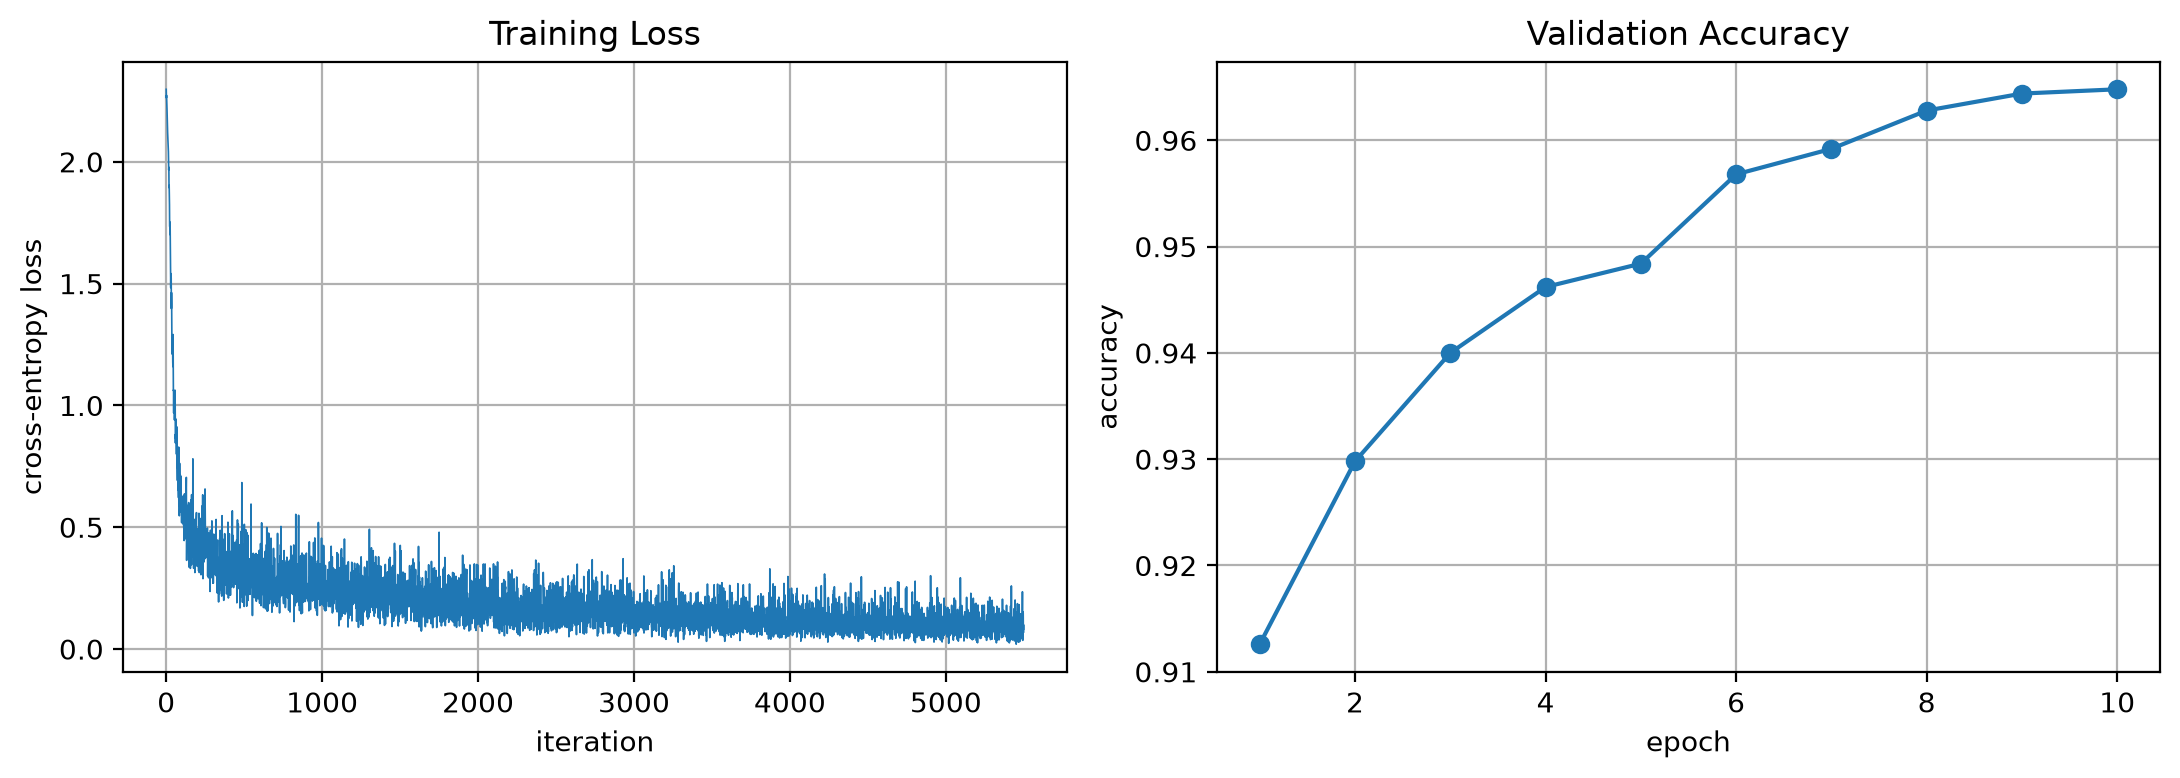
\includegraphics[width=0.92\linewidth]{torch_loss_acc.png}
\figcap{왼쪽: 미니배치마다의 손실 ($550\times10=5500$ iteration). 오른쪽: epoch마다의 검증 정확도}
\begin{itemize}
\item 손실은 처음에 빠르게 줄고, 미니배치마다 데이터가 달라서 \textbf{들쭉날쭉}하다 (확률적 경사하강법)
\item 검증 정확도는 아직 오르고 있다 $\to$ epoch를 늘리면 더 좋아질 수 있다
\end{itemize}
\end{frame}

\begin{frame}[fragile]{6. 결과 그림 (2): 예측 확인}
\begin{lstlisting}
model.eval()
with torch.no_grad():
    xb, yb = next(iter(test_loader))                     # first test mini-batch
    probs = torch.softmax(model(xb.to(device)), dim=1).cpu()
pred = probs.argmax(dim=1)
...
    a.imshow(xb[k].reshape(28, 28), cmap="gray")         # 784 -> 28 x 28
    a.set_title(f"pred {pred[k].item()}\n({probs[k, pred[k]]:.2f})", fontsize=8)
\end{lstlisting}
\centering
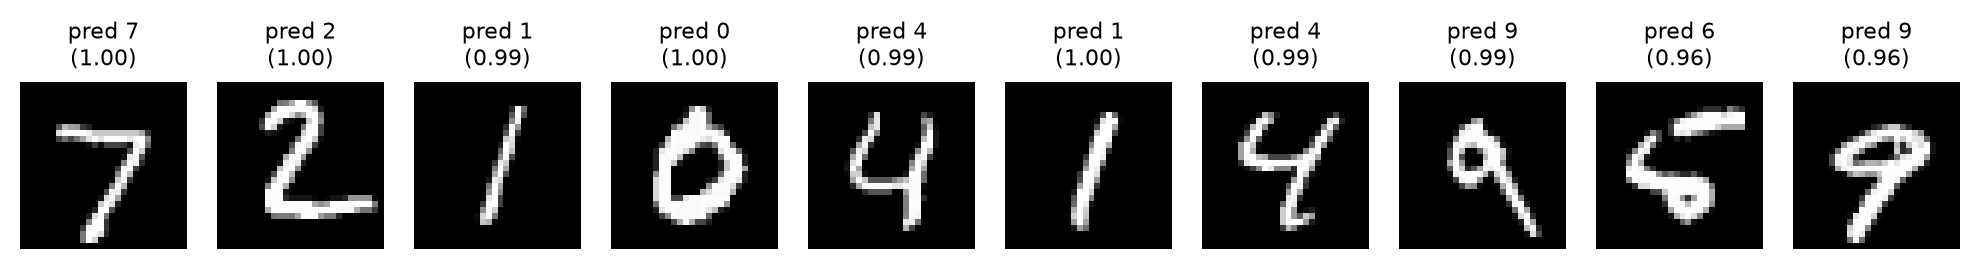
\includegraphics[width=0.95\linewidth]{torch_predictions.png}
\raggedright
\small
\begin{itemize}
\item \code{next(iter(test\_loader))}: DataLoader에서 첫 미니배치 하나만 꺼낸다
\item 확률이 필요하므로 여기서는 \code{torch.softmax}를 직접 쓴다. 그림을 그리려고 \code{.cpu()}로 가져온다
\end{itemize}
\end{frame}

\begin{frame}[fragile]{7. 학습한 모델 저장하고 다시 불러오기}
\textbf{저장} (\code{mnist\_torch.py}의 마지막 줄)
\begin{lstlisting}
torch.save(model.state_dict(), "mnist_mlp.pt")
\end{lstlisting}
\textbf{불러오기} (다른 프로그램에서)
\begin{lstlisting}
model2 = MLP(hidden=(100,))                          # the same structure first
model2.load_state_dict(torch.load("mnist_mlp.pt"))   # then the trained numbers
model2.eval()
\end{lstlisting}
\begin{itemize}
\item \code{state\_dict}: \code{\{"net.0.weight": ..., "net.0.bias": ..., "net.2.weight": ..., "net.2.bias": ...\}}
\item 저장되는 것은 \textbf{숫자(매개변수)뿐}이다. 구조는 코드(\code{class MLP})로 다시 만든다
\item 학습에 몇 시간, 며칠이 걸리는 모델도 한 번 저장해 두면 바로 예측에 쓸 수 있다
\item 공개된 학습된 모델을 내려받아 쓰는 것(전이학습)도 이 방법이다
\end{itemize}
\end{frame}

\begin{frame}{NumPy 버전과 무엇이 달라졌나}
\centering
\small
\renewcommand{\arraystretch}{1.12}
\begin{tabular}{>{\raggedright}p{3.0cm}>{\raggedright}p{4.9cm}>{\raggedright\arraybackslash}p{4.9cm}}
\toprule
& \textbf{NumPy (\code{mnist\_lab.py})} & \textbf{PyTorch (\code{mnist\_torch.py})} \\
\midrule
정답 표현 & one-hot \code{(N, 10)} & 클래스 번호 \code{(N,)}, \code{int64} \\
계층 & \code{Affine}, \code{Relu} 직접 작성 & \code{nn.Linear}, \code{nn.ReLU} \\
가중치 초기화 & 직접 (\code{0.01 * randn} 등) & 자동 \\
출력층 & \code{SoftmaxWithCrossEntropy} & \code{nn.CrossEntropyLoss} (logits 입력) \\
역전파 & 계층마다 \code{backward}, 기울기 검사 & \code{loss.backward()} \\
갱신 & \code{W -= lr * dW} & \code{optimizer.step()} \\
미니배치 & \code{permutation}으로 섞고 자르기 & \code{DataLoader(shuffle=True)} \\
GPU & 불가능 & \code{.to(device)} \\
\bottomrule
\end{tabular}
\vskip2mm
\raggedright
\begin{itemize}
\item 코드는 짧아졌지만 \textbf{하는 일은 같다}. 각 줄 뒤에서 무엇이 계산되는지 우리는 이미 알고 있다
\end{itemize}
\end{frame}

% =================================================
\section{정리와 실습}
% =================================================

\begin{frame}{정리}
\begin{keybox}[이번 시간의 핵심]
\small
\begin{itemize}\setlength{\itemsep}{0.6mm}
\item \textbf{텐서}: NumPy 배열 + GPU. 속성 \code{shape}, \code{dtype} (\code{float32}, 레이블은 \code{int64}), \code{device}
\item \textbf{자동 미분}: 순전파가 그래프를 기록하고 \code{loss.backward()}가 모든 \code{.grad}를 채운다.
기울기는 더해지므로 매번 \code{zero\_grad()}
\item \textbf{\code{nn}}: \code{nn.Module}을 상속하고 \code{forward}만 쓴다. \code{nn.Linear}의 가중치는 \code{(out, in)}
\item \textbf{\code{nn.CrossEntropyLoss}}: logits와 클래스 번호를 받는다. 모델에 softmax를 넣지 않는다
\item \textbf{\code{optim}}: \code{zero\_grad()}, \code{step()}
\item \textbf{\code{utils.data}}: \code{TensorDataset}, \code{random\_split}, \code{DataLoader}
\item \textbf{학습 루프 5줄}: 순전파 $\to$ 손실 $\to$ \code{zero\_grad} $\to$ \code{backward} $\to$ \code{step}
\item 평가할 때: \code{model.eval()}, \code{torch.no\_grad()}
\end{itemize}
\end{keybox}
\end{frame}

\begin{frame}[fragile]{같은 틀로 CNN도: 바꾸는 것은 모델뿐}
\begin{lstlisting}
model = nn.Sequential(
    nn.Conv2d(1, 16, kernel_size=3, padding=1),  # (N,1,28,28) -> (N,16,28,28)
    nn.ReLU(),
    nn.MaxPool2d(2),                             # -> (N,16,14,14)
    nn.Flatten(),                                # -> (N,3136)
    nn.Linear(16 * 14 * 14, 10),                 # -> (N,10)
).to(device)
\end{lstlisting}
\begin{itemize}
\item CNN 시간에 배운 계층들이 그대로 있다. 매개변수 $31530$개
\item 입력은 펼치지 않고 이미지 모양 그대로: \code{xb.reshape(-1, 1, 28, 28)}
\item 손실 함수, 최적화 기법, \code{train\_one\_epoch}, \code{evaluate}는 \textbf{한 글자도 바꾸지 않는다}
\end{itemize}
\end{frame}

\begin{frame}{실습 과제}
\small
\code{mnist\_torch.py}를 복사해서 하나씩 바꿔 보고, 검증 정확도와 test 정확도를 기록하자.
\begin{enumerate}
\item \textbf{epoch 평균 손실}을 출력하도록 고치기 (힌트: \code{np.mean})
\item 은닉층을 \code{hidden=(256, 128)}로 바꾸기. 매개변수 수는 몇 개인가? 손으로 먼저 계산해 보자
\item 최적화 기법을 \code{torch.optim.Adam(model.parameters(), lr=0.001)}로 바꾸기
\item \code{MLP} 클래스에 \code{nn.Dropout(0.2)}를 ReLU 뒤에 넣기. \code{model.train()}과 \code{model.eval()}의 역할을 설명하기
\item \code{optimizer.zero\_grad()}를 \textbf{지우고} 실행해 보기. 무슨 일이 생기고, 왜 그런가?
\item test 데이터 중 \textbf{틀린 이미지}를 찾아 예측과 정답을 함께 그리기
\item 앞 슬라이드의 CNN으로 모델을 바꾸기 (입력 \code{reshape}에 주의). MLP와 정확도 비교
\item 저장한 \code{mnist\_mlp.pt}를 새 프로그램에서 불러와 test 정확도가 같은지 확인하기
\end{enumerate}
\end{frame}

\end{document}
